\section{Modeling Recoil Bands}
Using the process described below, i will model the atomic recoil bands. Modeling the yield in atomic recoil events requires a knowledge of the charge and phonon resolution [kennedy thesis]. The resolution for electron and nuclear recoils were found by D. Jardin on CDMS iZIP data to be,

\begin{equation}
\sigma_E = \sqrt{\alpha +\beta E + \gamma E^2}
\end{equation}
\noindent
where $\alpha$ is a constant from electronic noise, $\beta E$ represents statistical variation, and $\gamma E^2$ is related to the contribution from noise and incomplete charge. The values for the constants are determined experimentally for the two different recoil types. $E$ is the energy of the recoil. The initial recoil energies are found through Monte Carlo, where the electron recoil energies are randomly drawn from an exponential distribution, and the nuclear recoil energies are drawn from a uniform distribution, 

\begin{equation}
\begin{gathered}
f(E_{er},\lambda) = \lambda e^{E_{er}\lambda}\\
f(E_{nr}) = \frac{1}{b-a}
\end{gathered}
\end{equation}
\noindent
where $\lambda$ is the rate parameter and $a$ and $b$ form the energy interval of interest. With the random energies drawn from the distributions above and the ionization yield calculated in equation 2.4, the total charge and phonon energies can be calculated. 

\begin{equation}
\begin{gathered}
E_Q = YE_R\\
E_T = [1 + Y\frac{eV}{\epsilon}]E_R
\end{gathered}
\end{equation} 
The energies are used to determine the resolution defined by equation 2.6. A normal distribution is formed with the newly defined resolution and randomly sampled. This randomly sampled energy is added to the previously calculated energy. The recoil energies calculated are what is expected to be measured. Using the expected energies, the expected ionization yield need to be calculated.

\begin{equation}
\begin{gathered}
Y = \frac{E_Q}{E_T-\frac{eV}{\epsilon}E_Q}
\end{gathered}
\end{equation}



\begin{figure}[h]
	\centering
	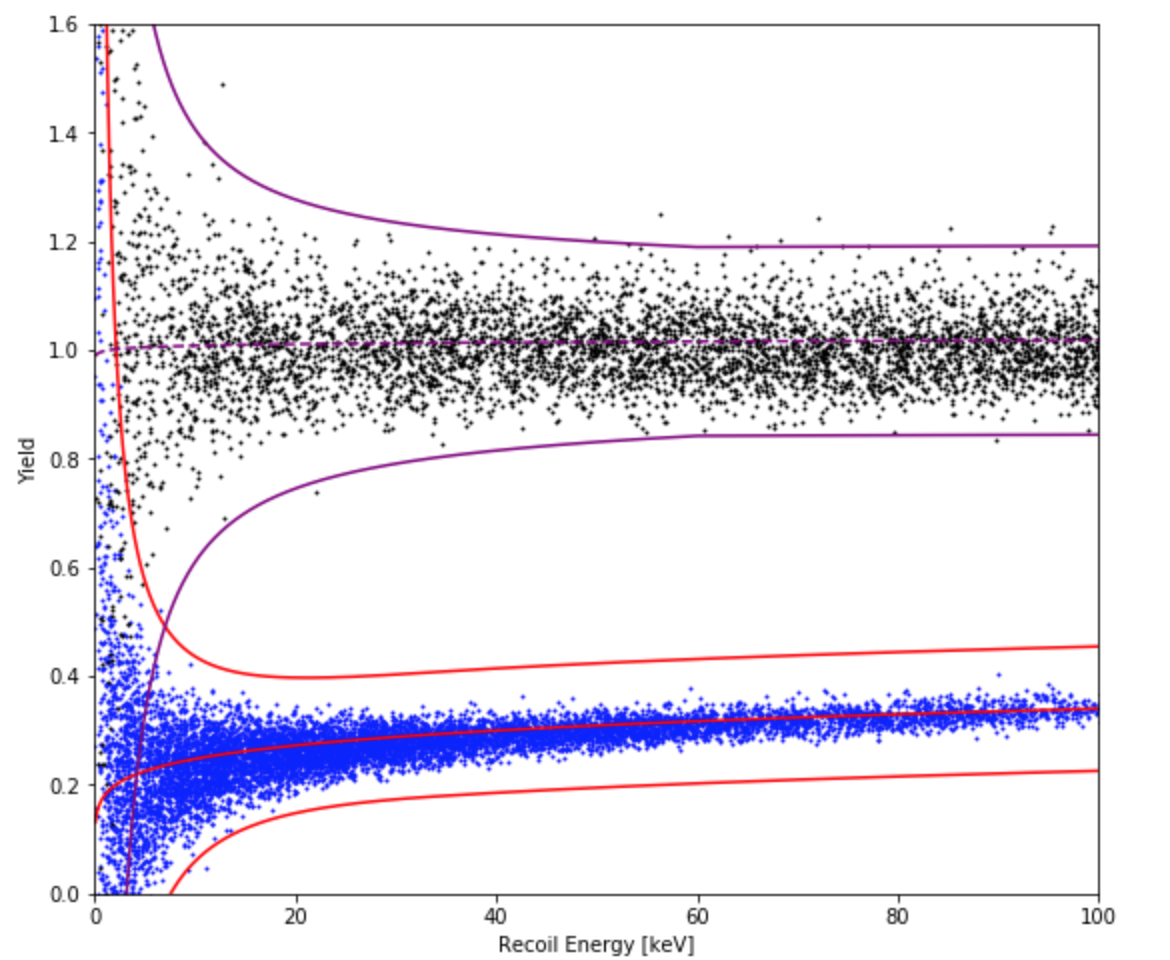
\includegraphics[scale=.5]{Sim_Bands}
	\caption{Simultaed Recoil Bands}
\end{figure}
\noindent
Plotting the expected recoil energies versus the expected ionization yield creates the recoil bands shown in figure 3.1. Comparing figure 2.2 with figure 3.1, there is a distinct difference in the width of the bands, with the more extreme case shown in the nuclear recoil band pictured in blue. 
\\
The purpose of the process outlined above is to recreate the electronic and nuclear recoil bands with an added "fano factor" to the variance. The fano factor will be added in a fashion similar to equation 2.7, but instead of a functional form dependent upon the energy, it will be a random constant. Once the bands with a fano factor are simulated, I will write a program to extract the fano factor from the width of the data. Extracting the fano factor will be done by breaking the data into logarithmically spaced bins and fitting the data in the bins to determine the width. The data in each bin is assumed to be approximately normally distributed. Successfully extracting the fano factor added to the simulated data will allow the extraction of a fano factor from real data, which will help give a more accurate determination of a fano factor that should be added to the simulation. \par
\noindent
When a comfortable value for a the fano factor is determined. I will try to accurately model californium data. Doing so should give a good idea of how well a fano factor accurately explains the difference in the variance from data to model. The factor is not going to just be one number. This is due to the possible energy dependence. This should allow me to give a good "bound" on what the possible fano factors can be. \par
\noindent
Something that i would like to do is to determine a functional form of the fano factor from the data. This should give a better understanding of what the actualence of the variance is; as shown above there a different expected fucntional forfunctional variance. I would then like to compare this to what Lindhard predicts for the variance. 






\section{Lindhard Variance Calculation}
The Lindhard variance is not something that is easily calculated. Equation 2.8 is the definition of variance, but involves first solving equation 2.1. Equation 2.1 is what is called a " non-linear integral differential equation." These equations cannot be solved analytically and therefor must be solved using a numerical quadrature algorithm combined with an accurate and efficient ODE solver. \cite{IDEQ} Once solved, the variance equation needs to be solved using the same method with the result from solving equation 2.1.

\begin{equation}
\begin{gathered}
k \epsilon^{1/2}\frac{d\Omega^2}{\epsilon}(\epsilon) = \int_{0}^{\epsilon^{2}} \frac{dt}{2t^{\frac{3}{2}}}f(t^{1/2})(\Omega^2(\epsilon -\frac{t}{\epsilon}) - \Omega^2(\epsilon) +\Omega^2(\frac{t}{\epsilon})) +\dots\\
\int_{0}^{\epsilon^{2}} \frac{dt}{2t^{\frac{3}{2}}}f(t^{1/2})(\nu(\epsilon -\frac{t}{\epsilon}) - \nu(\epsilon)+\nu(\frac{t}{\epsilon}))
\end{gathered}
\end{equation}

\noindent
Once the method to solve this is figured out, the variance can be added to the simulation and then be compared to the data, and the fano factor method. 

\noindent
\textbf{I am still uncertain how i am going to compared to data. Perhaps i should mention that is what i need to figure out? Or is that straight forward? }